\resizebox{\textwidth}{!}{
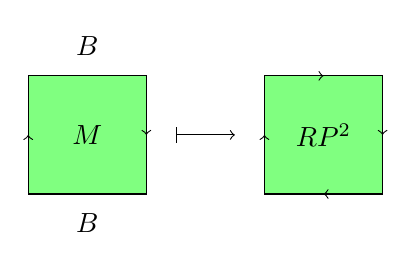
\begin{tikzpicture}[scale=1.5]

\draw[fill=green!50] (0,0) -- (0,1) -- (1,1) -- (1,0) -- cycle;
\draw[-to] (0,0) -- (0,0.5);
\draw[-to] (1,1) -- (1,0.5);
\draw (0.5,0.5) node {$M$};
\draw (0.5,1.25) node {$B$};
\draw (0.5,-.25) node {$B$};

\draw[|-to] (1.25,.5) -- (1.75,.5);

\draw[fill=green!50] (2,0) -- (2,1) -- (3,1) -- (3,0) -- cycle;
\draw[-to] (2,0) -- (2,.5);
\draw[-to] (2,1) -- (2.5,1);
\draw[-to] (3,1) -- (3,.5);
\draw[-to] (3,0) -- (2.5,0);
\draw (2.5,.5) node {$\mb{R}P^2$};

\end{tikzpicture}
}
